% exercise sheet with header on every page for math or close subjects
\documentclass[12pt]{article}
\usepackage[utf8]{inputenc} 
\usepackage{latexsym} 
\usepackage{multicol}
\usepackage{fancyhdr}
\usepackage{amsfonts} 
\usepackage{amsmath}
\usepackage{amssymb}
\usepackage{enumerate}
\usepackage{listings}
\usepackage{graphicx}
\usepackage{pdfpages}

% Shortcuts for bb, frak and cal letters
\newcommand{\E}{\mathbb{E}}
\newcommand{\V}{\mathbb{V}}
\renewcommand{\P}{\mathbb{P}}
\newcommand{\N}{\mathbb{N}}
\newcommand{\R}{\mathbb{R}}
\newcommand{\C}{\mathbb{C}}
\newcommand{\Z}{\mathbb{Z}}
\newcommand{\Pfrak}{\mathfrak{P}}
\newcommand{\Pfrac}{\mathfrak{P}}
\newcommand{\Bfrac}{\mathfrak{P}}
\newcommand{\Bfrak}{\mathfrak{B}}
\newcommand{\Fcal}{\mathcal{F}}
\newcommand{\Ycal}{\mathcal{Y}}
\newcommand{\Bcal}{\mathcal{B}}
\newcommand{\Acal}{\mathcal{A}}

% formating
\topmargin -1.5cm 
\textheight 24cm
\textwidth 16.0 cm 
\oddsidemargin -0.1cm

% Fancy Header on every Page
\pagestyle{fancy}
\lhead{\textbf{Programmierung for Engineers - Exercise 5}}
\rhead{Daniel Schäfer (2549458)\\ Dominik Weber (2548553)\\ Sina Vaghiri (2533563)}
\renewcommand{\headrulewidth}{1.2pt}
\setlength{\headheight}{60pt} 

\begin{document}
\pagenumbering{gobble}
\lstset{language=C}

\section{Aufgabe 1}
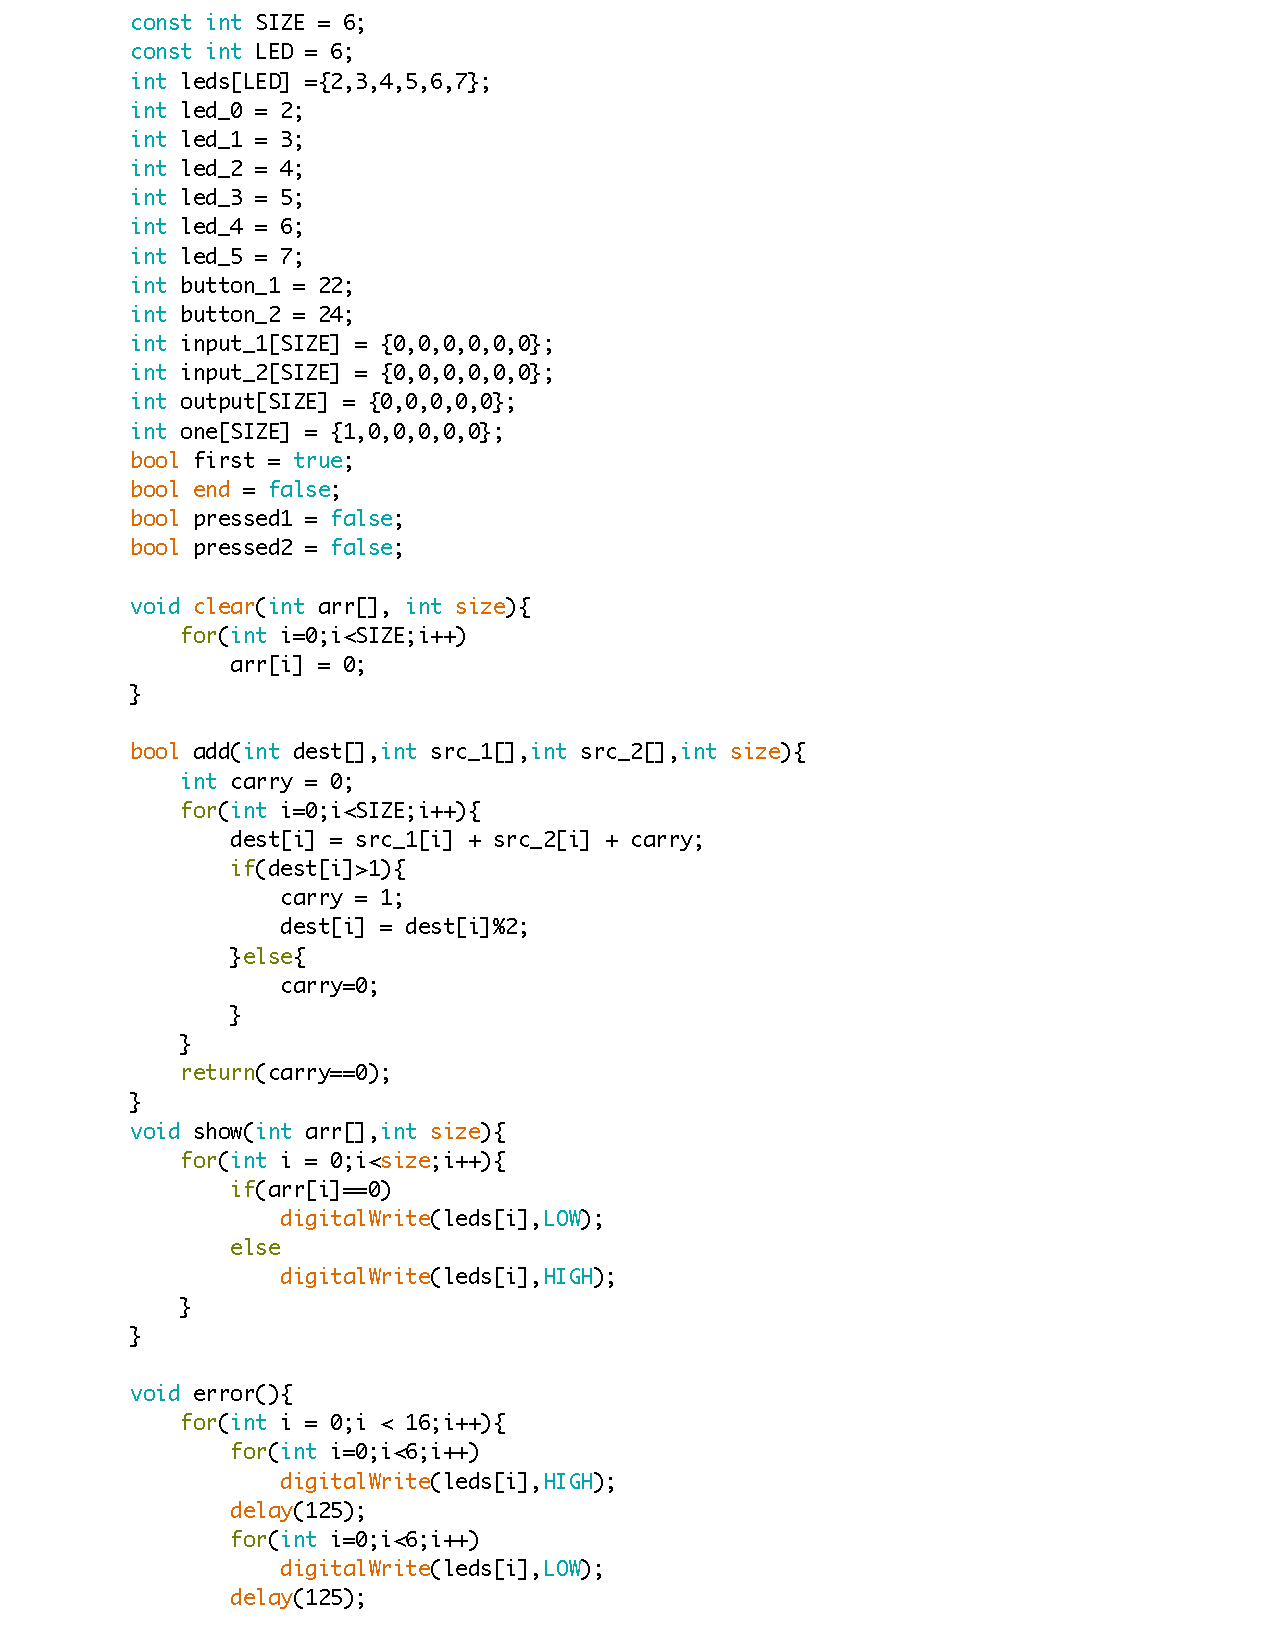
\includepdf[pages=-]{../Aufgabe1/Aufgabe1.pdf}

\section{Aufgabe 2}
\begin{enumerate}[1)]
    \item 
        It will print 12, because the local variable definition overwrites the global one.
    \item
        It will print 12, because the global variable was changed to 12 before the print happened.
    \item
        It will print the unchanged global variable 7, because the new local Variable x overwrites the global declaration of x only inside the brackets (which only contain the declaration). After leaving this scope, x references the global variable x = 7 again
    \item
        It will print the unchanged global variable 7, because the function alternate creates a new local variable x (in the scope of alternate) which gets ``thrown away'' after leaving the function altternate. 
    \item
        This time it will print the new global variable value 12, because the function alternate does not create a new local variable x this time, instead it writes inside the global variable x. the global variable gets changed to 12 and then printed.
\end{enumerate}


\end{document}
